%Jennifer Pan, August 2011

\documentclass[10pt,letter]{article}
	% basic article document class
	% use percent signs to make comments to yourself -- they will not show up.

\usepackage{amsmath}
\usepackage{amssymb}
	% packages that allow mathematical formatting

\usepackage[final]{graphicx}
\usepackage{caption}
\usepackage{subcaption}
\usepackage{subcaption}
	% package that allows you to include graphics
\usepackage{tikz}
\usepackage{setspace}
	% package that allows you to change spacing

\onehalfspacing
	% text become 1.5 spaced

\usepackage{fullpage}
	% package that specifies normal margins

\renewcommand{\vector}[1]{\boldsymbol{#1}}
\newcommand{\problem}[1]{\section*{Problem #1}}
\newcommand{\problempart}[1]{\paragraph{#1}}

\begin{document}
	% line of code telling latex that your document is beginning


\title{ECON 511 Problem Set 9}

\author{Nicholas Wu}

\date{Spring 2021}
	% Note: when you omit this command, the current dateis automatically included

\maketitle
	% tells latex to follow your header (e.g., title, author) commands.
%\textbf{Note:} I use bold symbols to denote vectors and nonbolded symbols to denote scalars. I primarily use vector notation to shorthand some of the sums, since many of the sums are dot products.

\problem{1}
My code only needs the data file in the MATLAB path and the hpfilter function from spatial econometrics.


\problempart{7} See the plots, figures 1-7.
\begin{figure}
\begin{center}
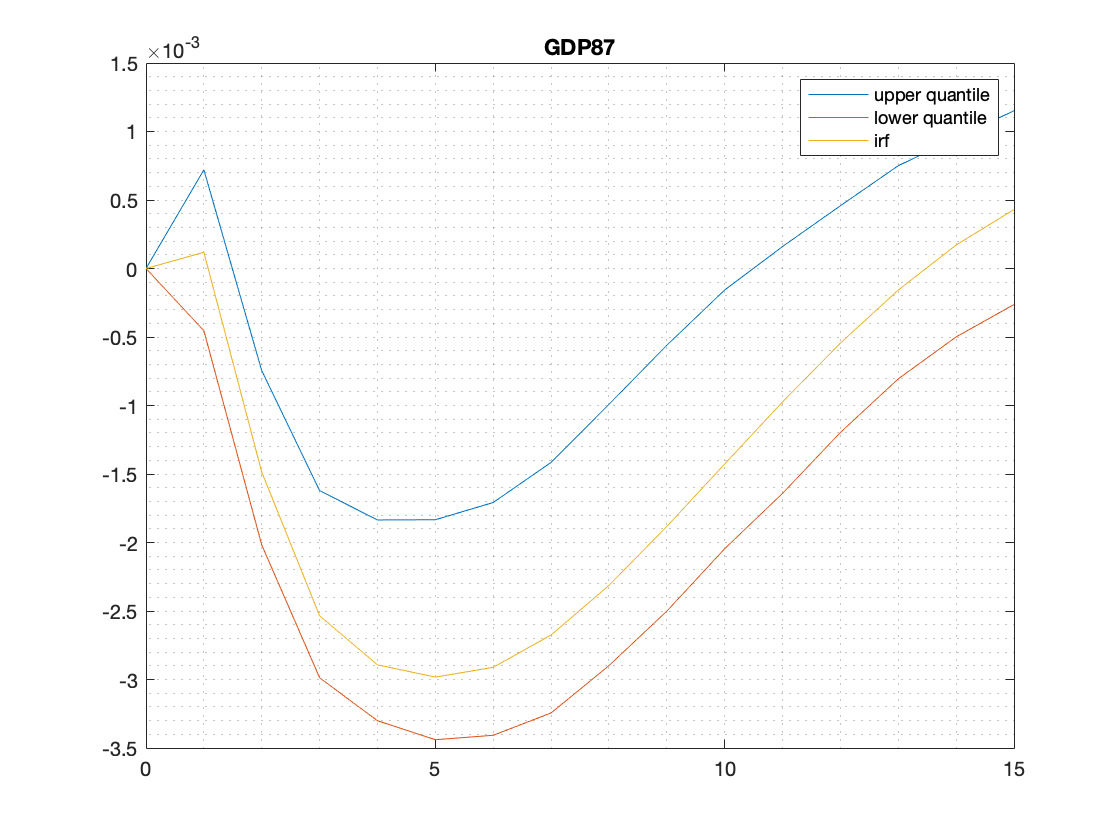
\includegraphics[width=15cm]{ps9fig1}
\caption{Part 7: IRF in GDP87}
\end{center}
\end{figure}
\begin{figure}
\begin{center}
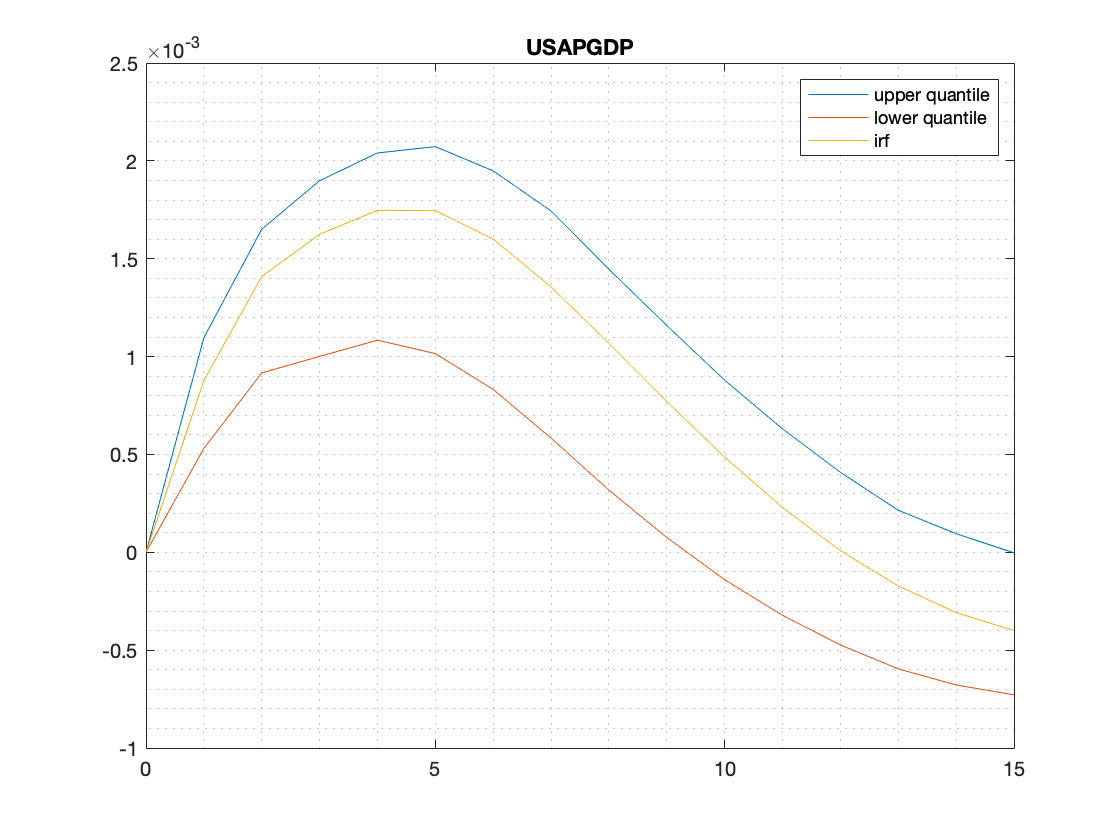
\includegraphics[width=15cm]{ps9fig2}
\caption{Part 7: IRF in USAPGDP}
\end{center}
\end{figure}
\begin{figure}
\begin{center}
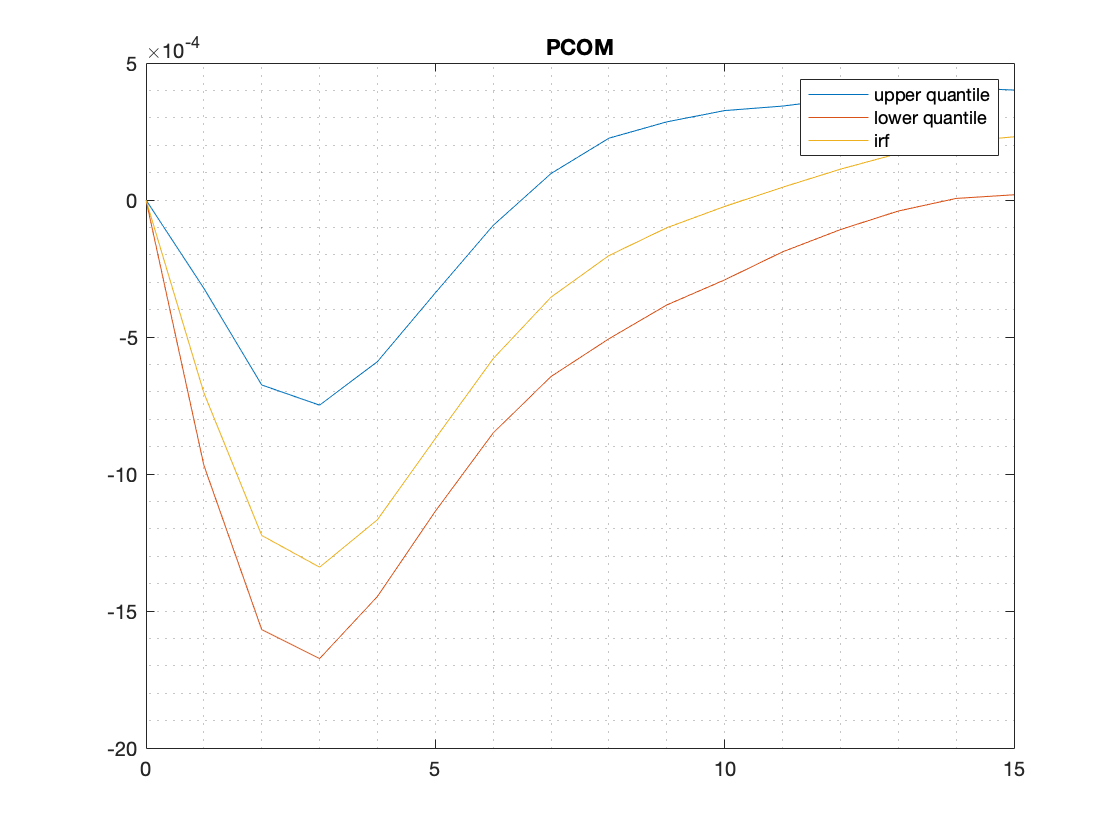
\includegraphics[width=15cm]{ps9fig3}
\caption{Part 7: IRF in PCOM}
\end{center}
\end{figure}
\begin{figure}
\begin{center}
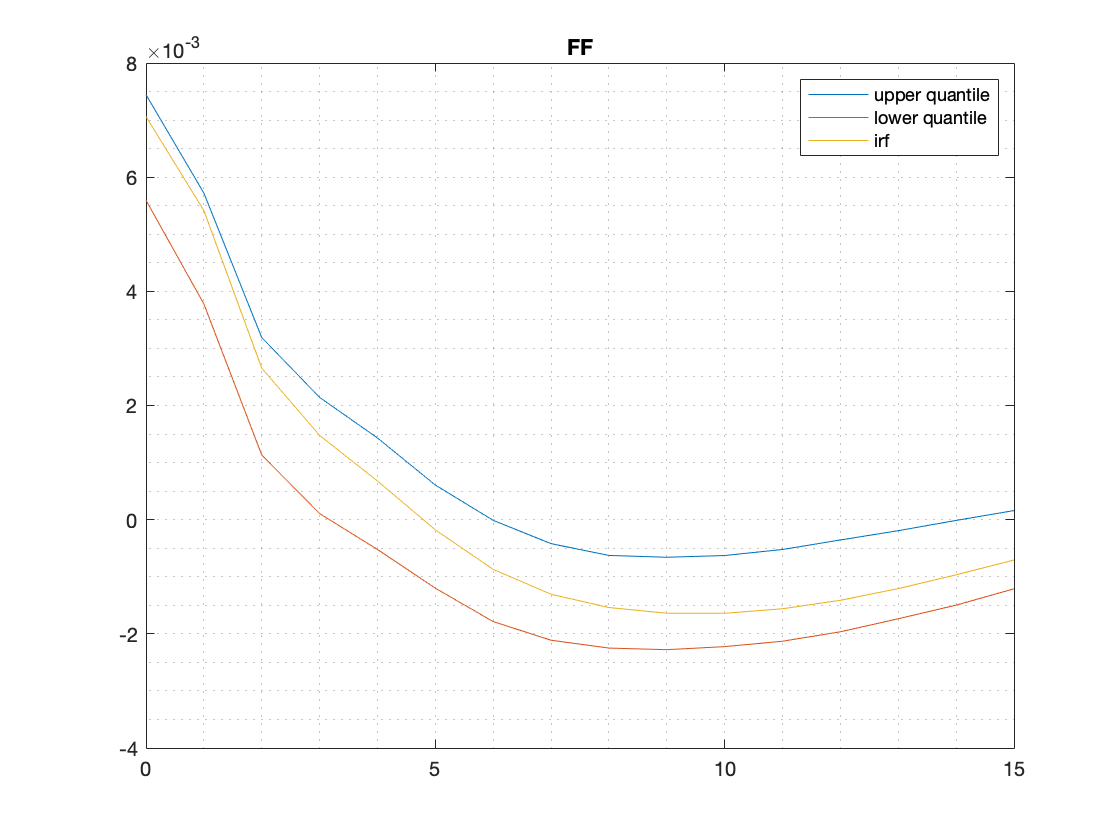
\includegraphics[width=15cm]{ps9fig4}
\caption{Part 7: IRF in FF}
\end{center}
\end{figure}
\begin{figure}
\begin{center}
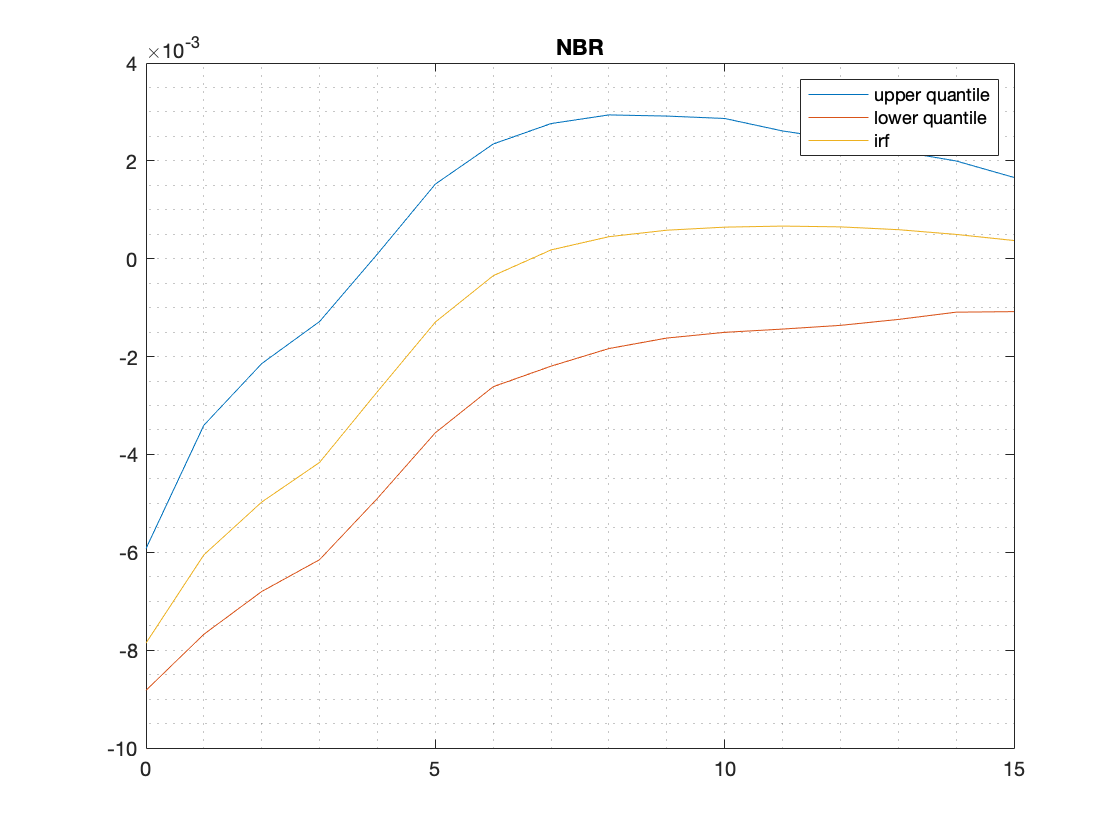
\includegraphics[width=15cm]{ps9fig5}
\caption{Part 7: IRF in NBR}
\end{center}
\end{figure}
\begin{figure}
\begin{center}
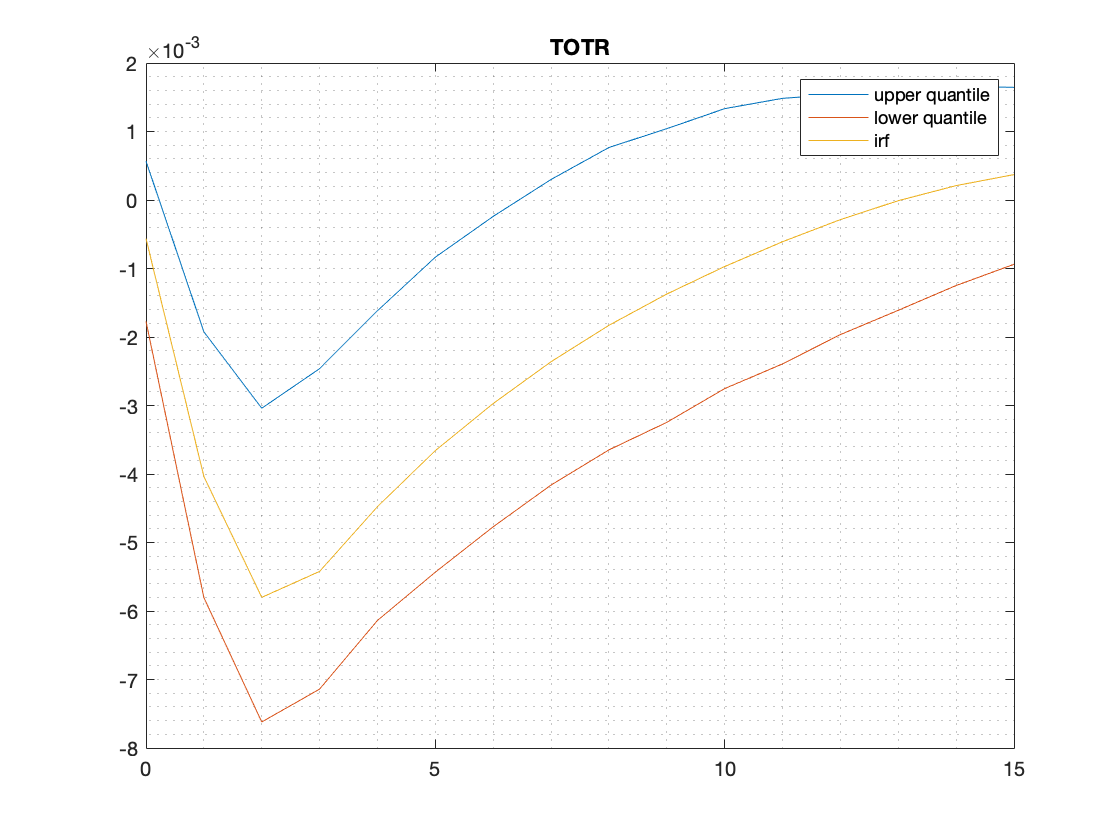
\includegraphics[width=15cm]{ps9fig6}
\caption{Part 7: IRF in TOTR}
\end{center}
\end{figure}
\begin{figure}
\begin{center}
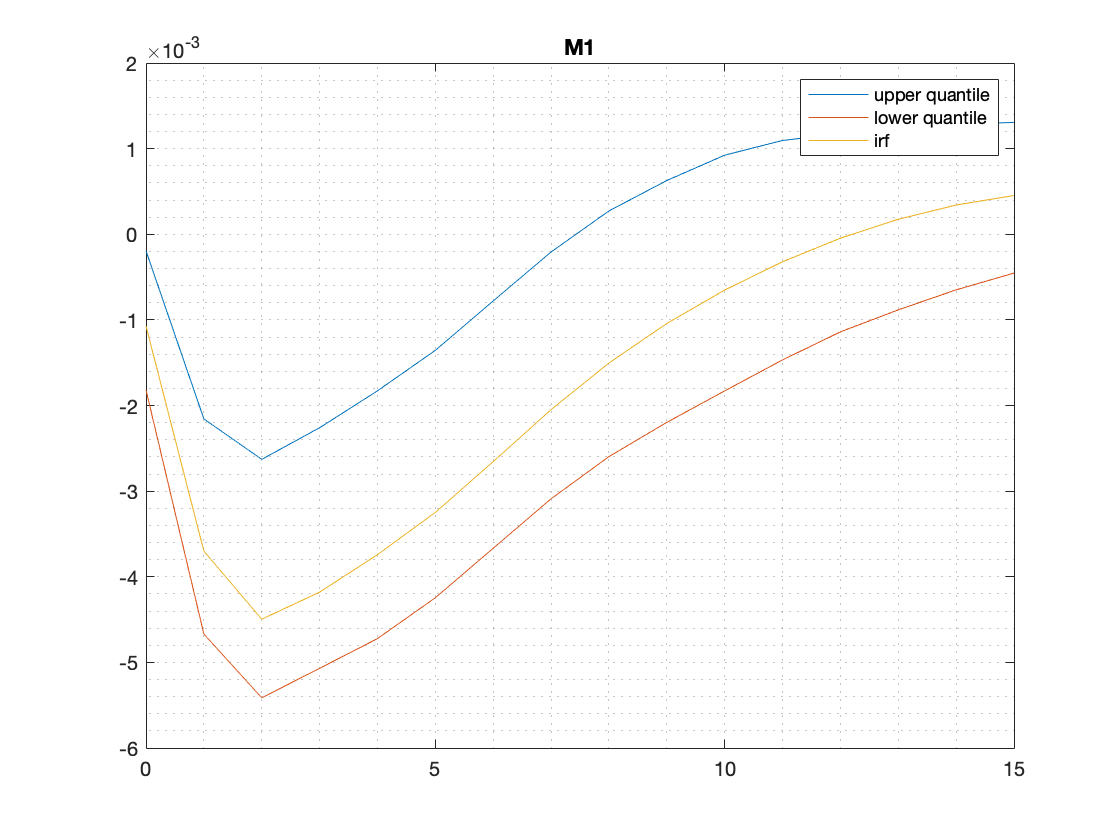
\includegraphics[width=15cm]{ps9fig7}
\caption{Part 7: IRF in M1}
\end{center}
\end{figure}

\problempart{8} The FF shock depresses output for $\approx$ 13 quarters. M1, PCOM, and TOTR decline significantly for a few quarters, and then recover. NBR drops immediately, but recovers. We also observe the price puzzle mentioned in lecture, the counterintuitive increase in inflation.

\problempart{9} See figures 8-10. These show the impulse responses to GDP87 only using portions of the data. Comparing these to figure 1, we note that the shapes of the impulse responses are similar, but not identical. (Similar observations can be made looking at the impulse responses for the other variables). The VAR assumption is that the structure of the relation does not change over time. In a very general sense, this is reasonable; these impulse responses are similar enough in shape to the impulse response estimated on the entire dataset, but we have to be cautious about quantitative analysis, since the exact magnitudes and persistences of these responses are not identical; when using the first half, the persistence of the shock is around 9 quarters, but on the second half, the persistence is around 15 quarters. Similarly, dropping the first 10 and last 10 gives a persistence of around 12 quarters, slightly less than using the entire time series.
\begin{figure}
\begin{center}
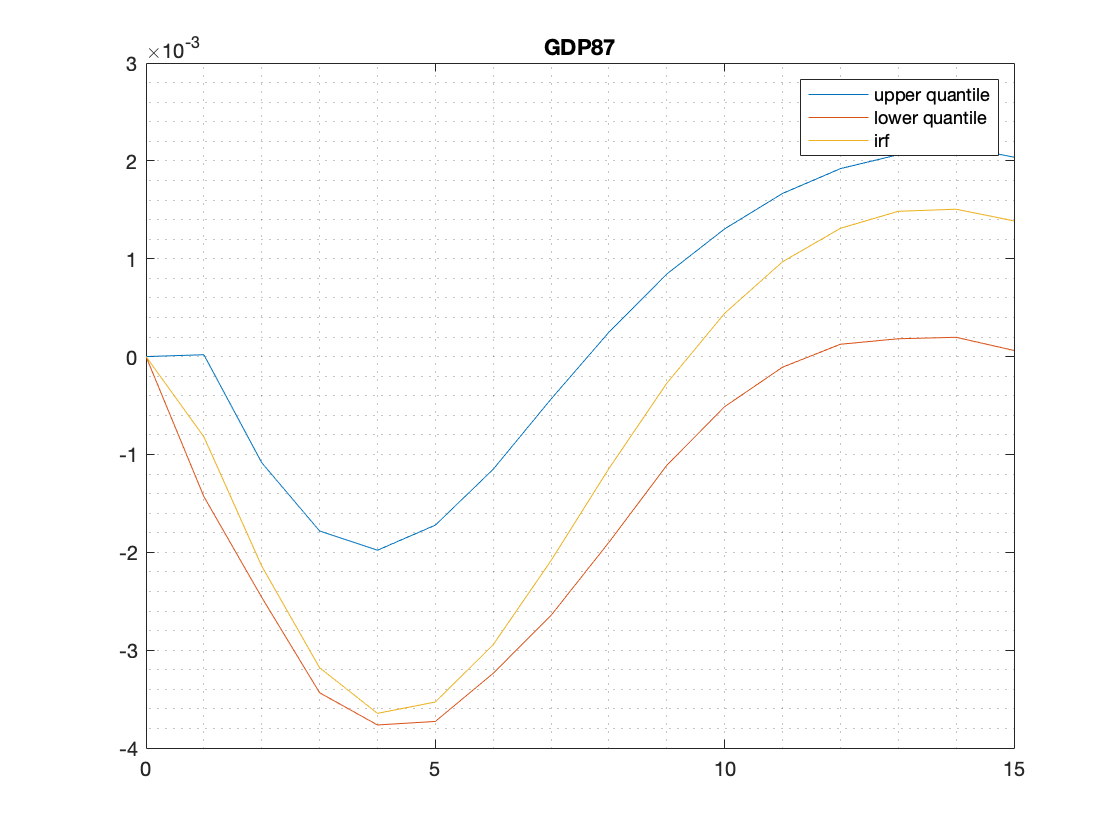
\includegraphics[width=15cm]{ps9fig8}
\caption{Part 9: IRF in GDP87, only using first half}
\end{center}
\end{figure}
\begin{figure}
\begin{center}
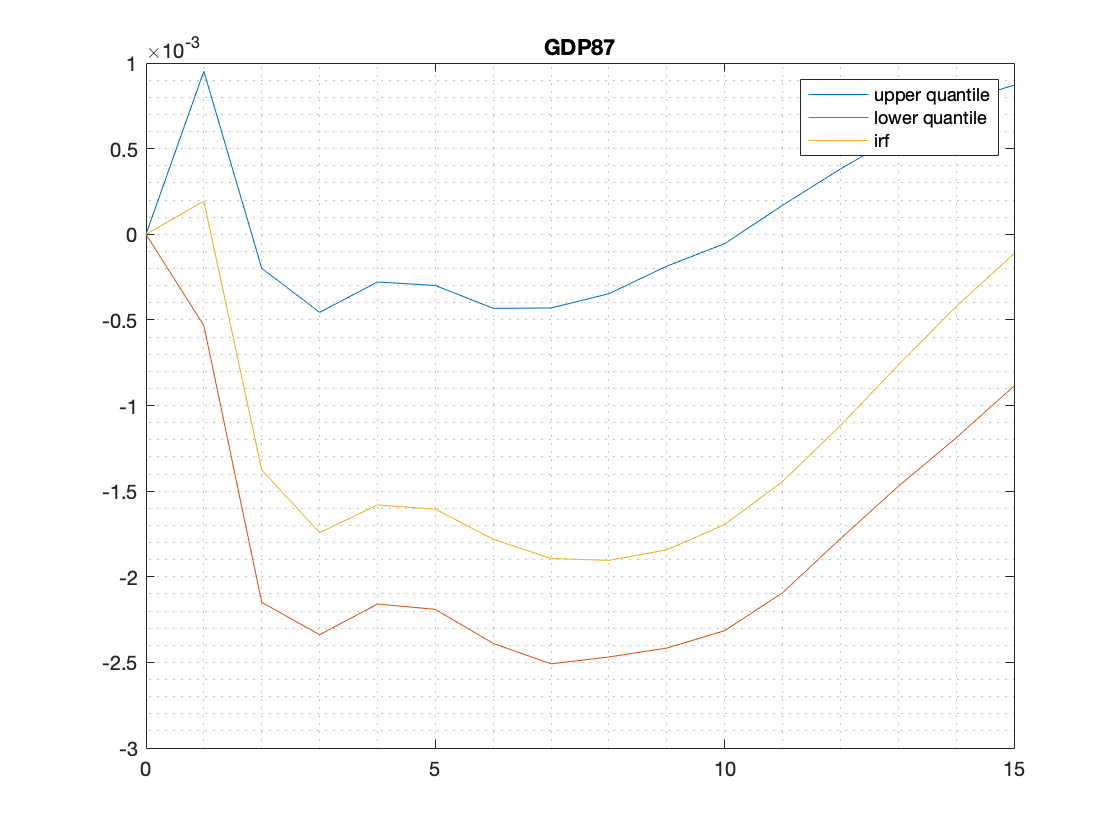
\includegraphics[width=15cm]{ps9fig9}
\caption{Part 9: IRF in GDP87, only using second half}
\end{center}
\end{figure}
\begin{figure}
\begin{center}
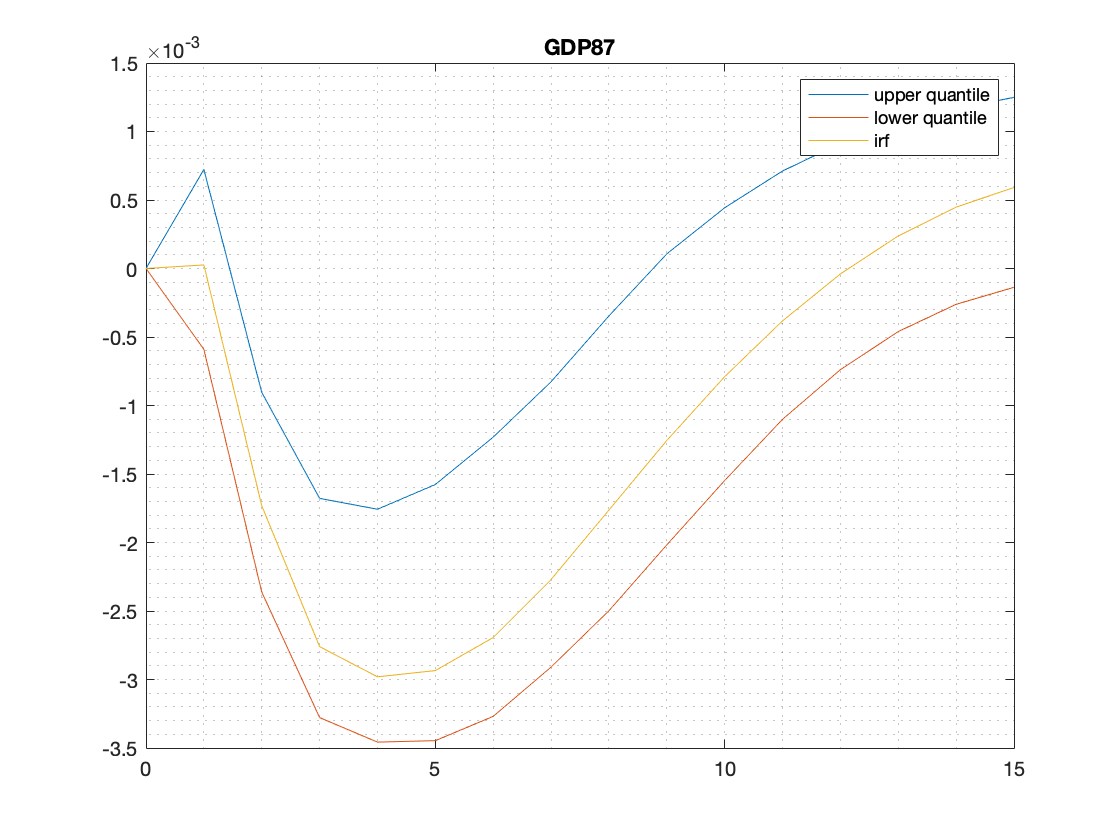
\includegraphics[width=15cm]{ps9fig10}
\caption{Part 9: IRF in GDP87, dropping first 10 and last 10}
\end{center}
\end{figure}
\problempart{10} Yes. Compare figure 11 with figure 1, showing the impulse responses of GDP87 in the event of a larger shock. Note the trough is roughly 5 times (proportial to the size of the shock) lower than the original case, thus suggesting that output reacts proportionally to shocks. This is due to the fact that the VAR is a linear model.
\begin{figure}
\begin{center}
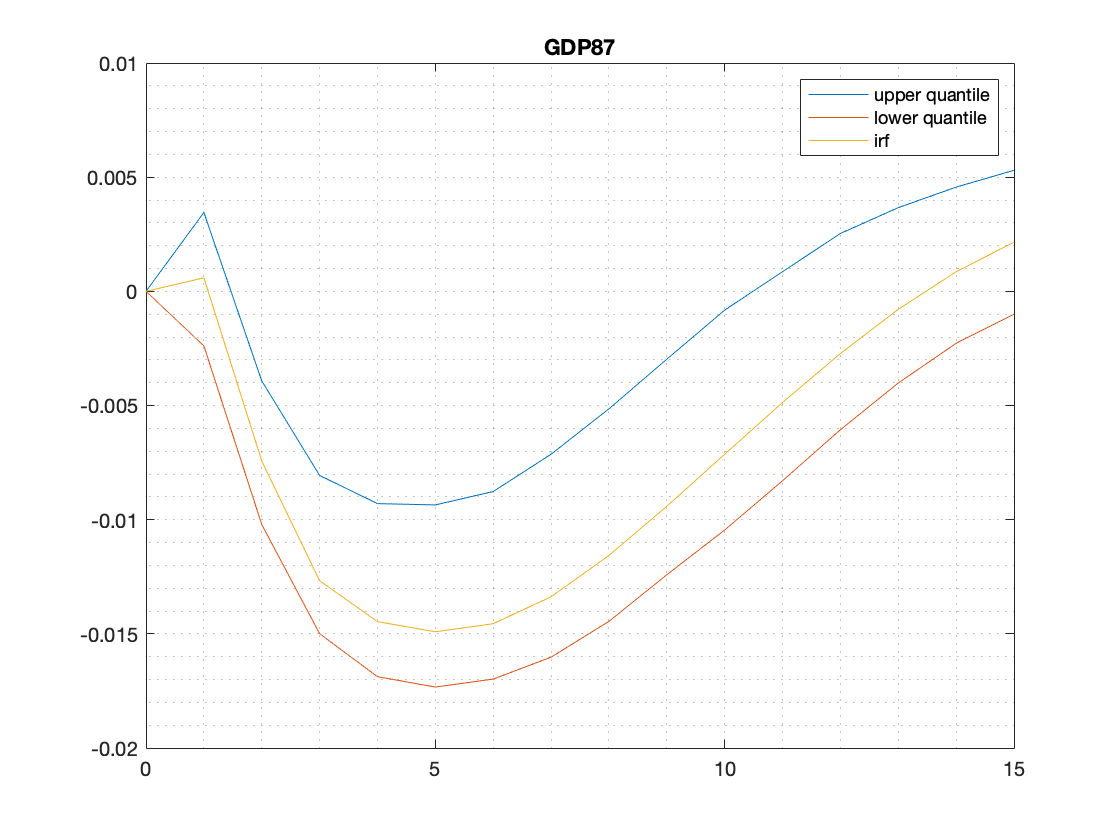
\includegraphics[width=15cm]{ps9fig11}
\caption{Part 10: IRF in GDP87, with a 0.05 shock rather than 0.01}
\end{center}
\end{figure}
\problempart{11} See figures 12 and 13. In the normal ordering, USAPGDP takes one quarter to react to an FF shock, but reacts immediately in the swapped order. Similarly, FF reacts immediately to a price shock in the normal ordering, but takes one quarter to react in the swapped order.

\begin{figure}
\centering
\begin{subfigure}[b]{0.45\textwidth}
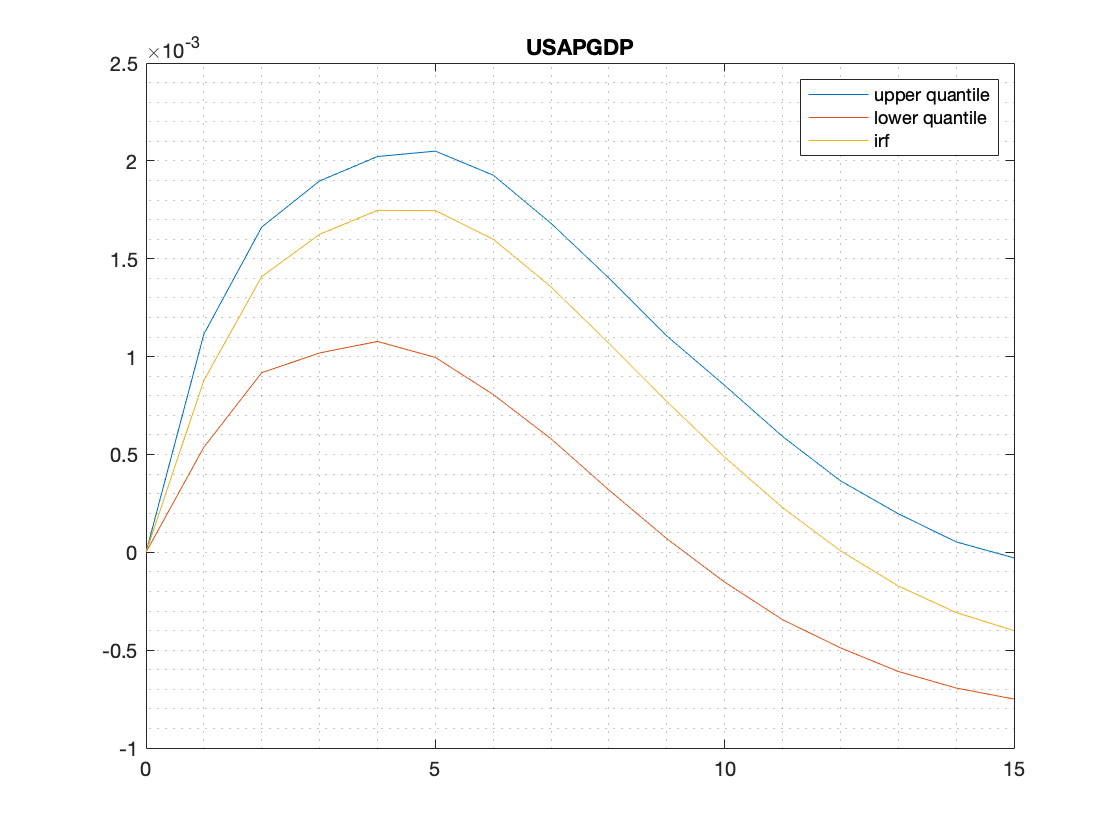
\includegraphics[width=7cm]{ps9fig12}
\caption{IRF USAPGDP, Normal, FF shock}
\end{subfigure}
\hfill
\begin{subfigure}[b]{0.45\textwidth}
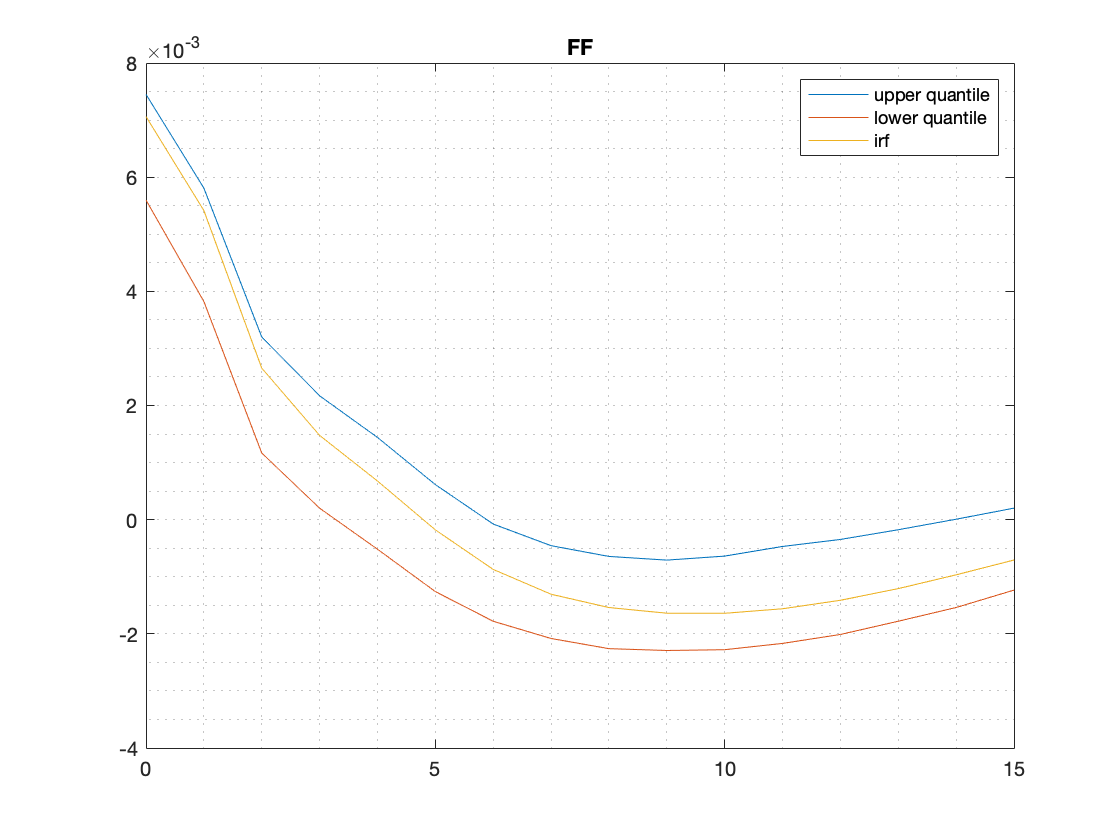
\includegraphics[width=7cm]{ps9fig12_2}
\caption{IRF FF, Normal, FF shock}
\end{subfigure}
\begin{subfigure}[b]{0.45\textwidth}
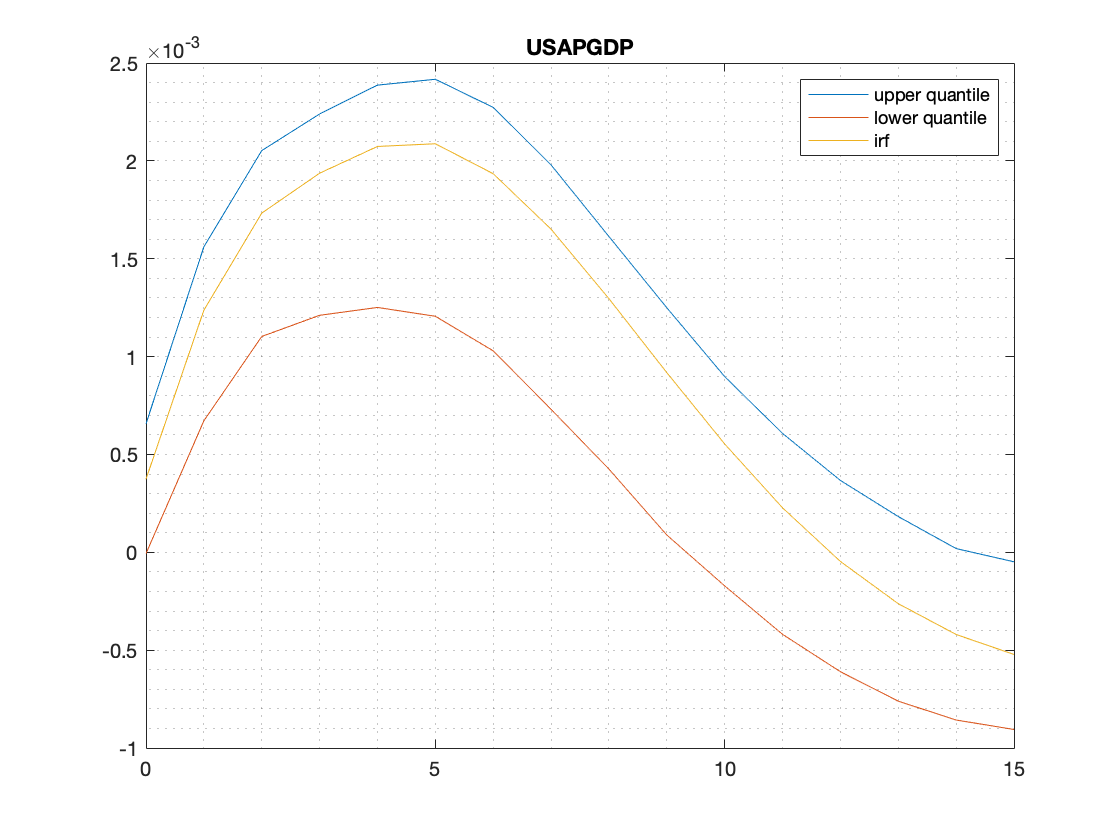
\includegraphics[width=7cm]{ps9fig12_3}
\caption{IRF USAPGDP, Swapped, FF shock}
\end{subfigure}
\hfill
\begin{subfigure}[b]{0.45\textwidth}
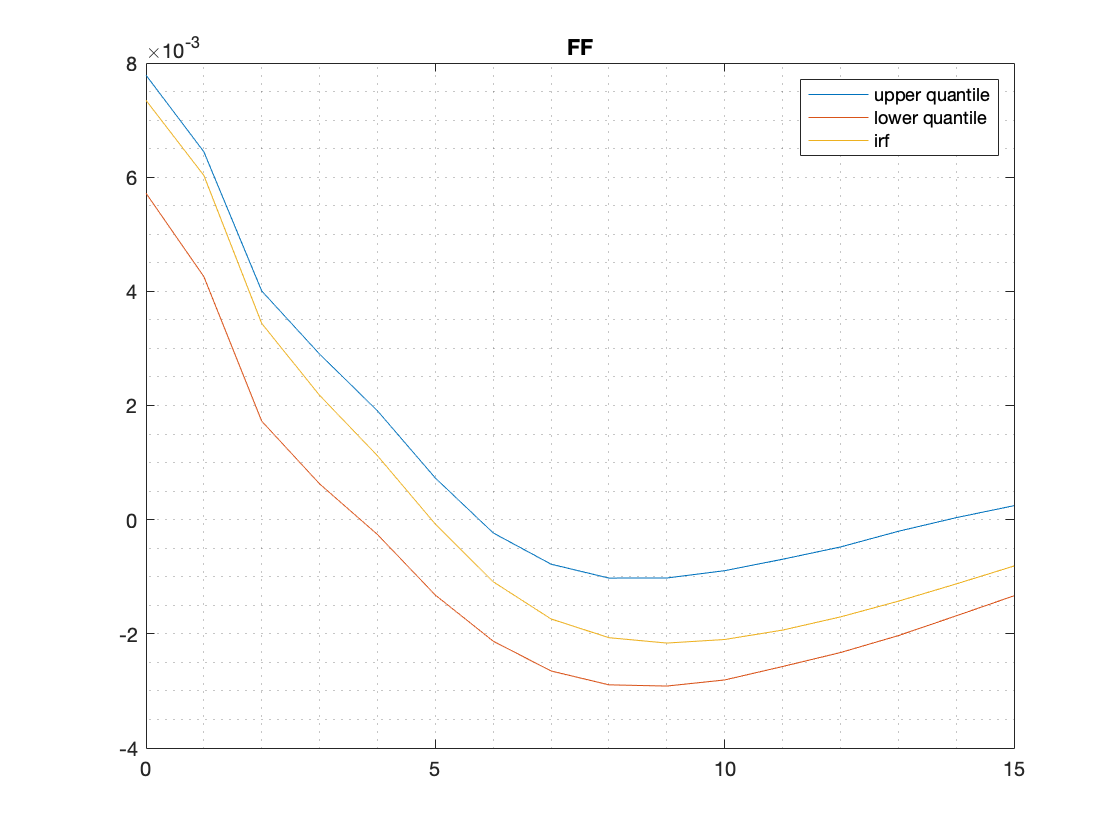
\includegraphics[width=7cm]{ps9fig12_4}
\caption{IRF FF, Swapped, FF shock}
\end{subfigure}
\caption{Part 11: FF shock, swapped and normal ordering.}
\end{figure}

\begin{figure}
\centering
\begin{subfigure}[b]{0.45\textwidth}
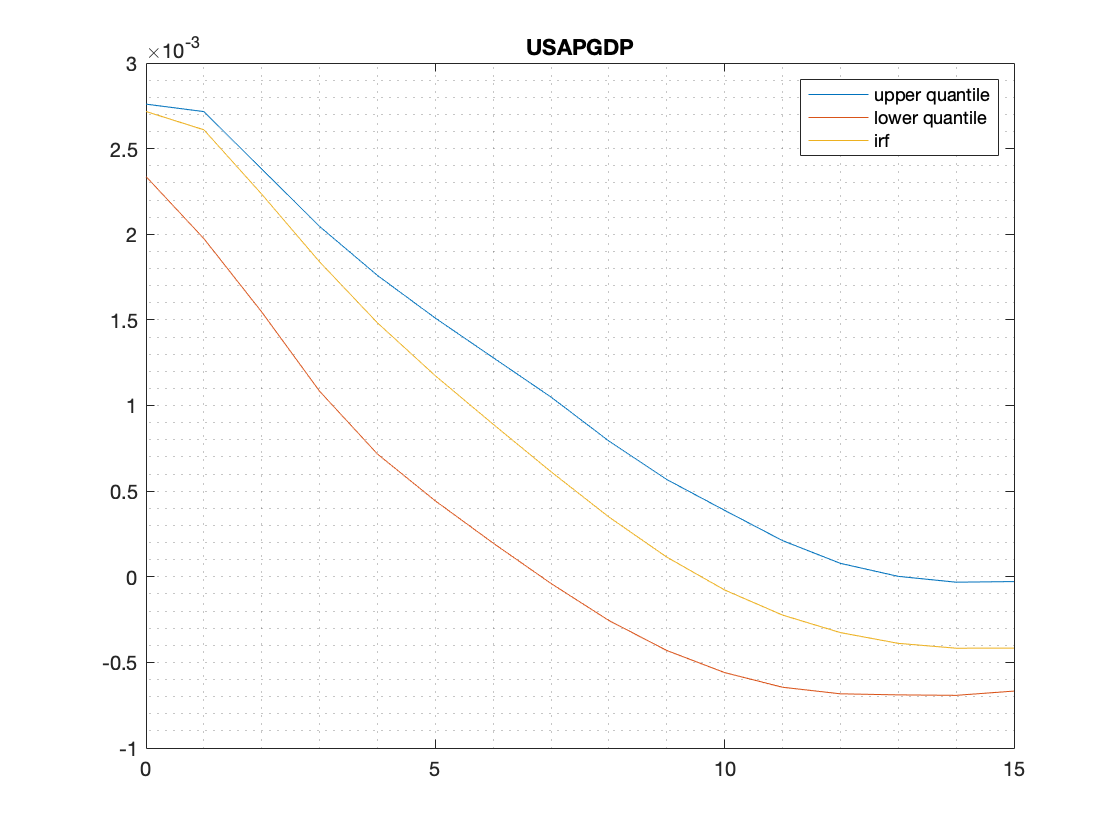
\includegraphics[width=7cm]{ps9fig13}
\caption{IRF USAPGDP, Normal order}
\end{subfigure}
\hfill
\begin{subfigure}[b]{0.45\textwidth}
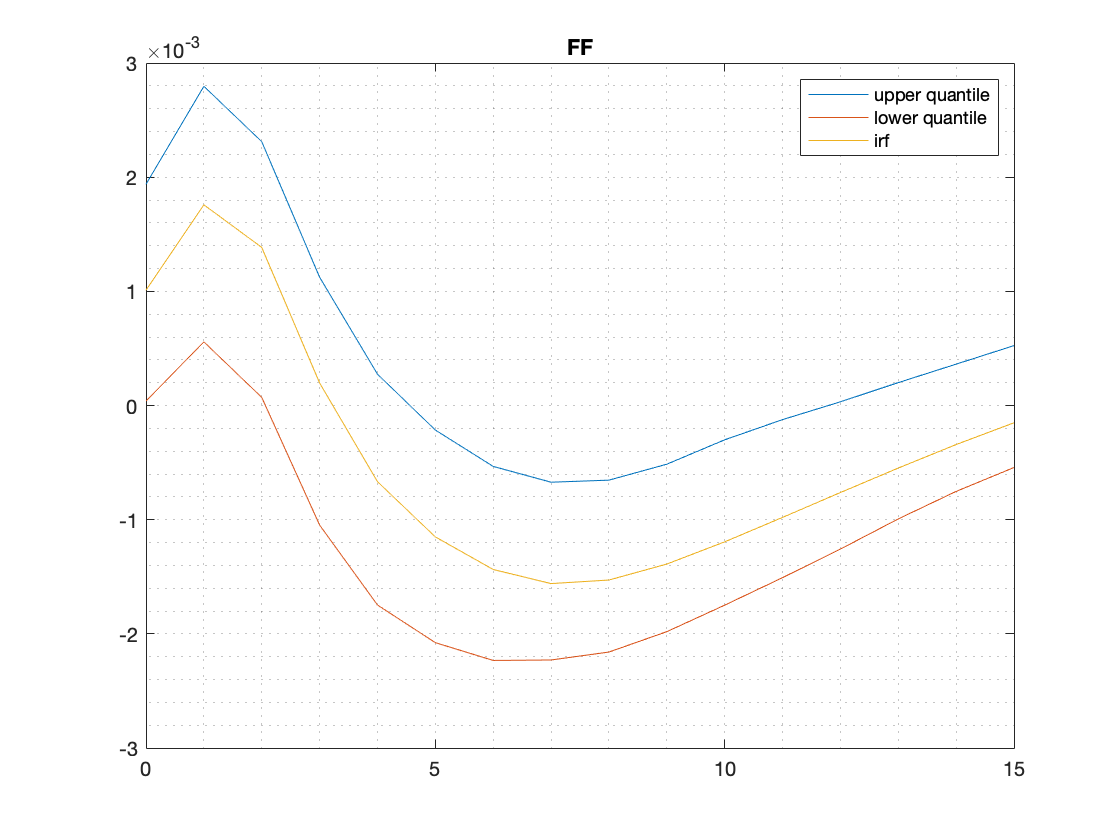
\includegraphics[width=7cm]{ps9fig13_2}
\caption{IRF FF, Normal order}
\end{subfigure}
\begin{subfigure}[b]{0.45\textwidth}
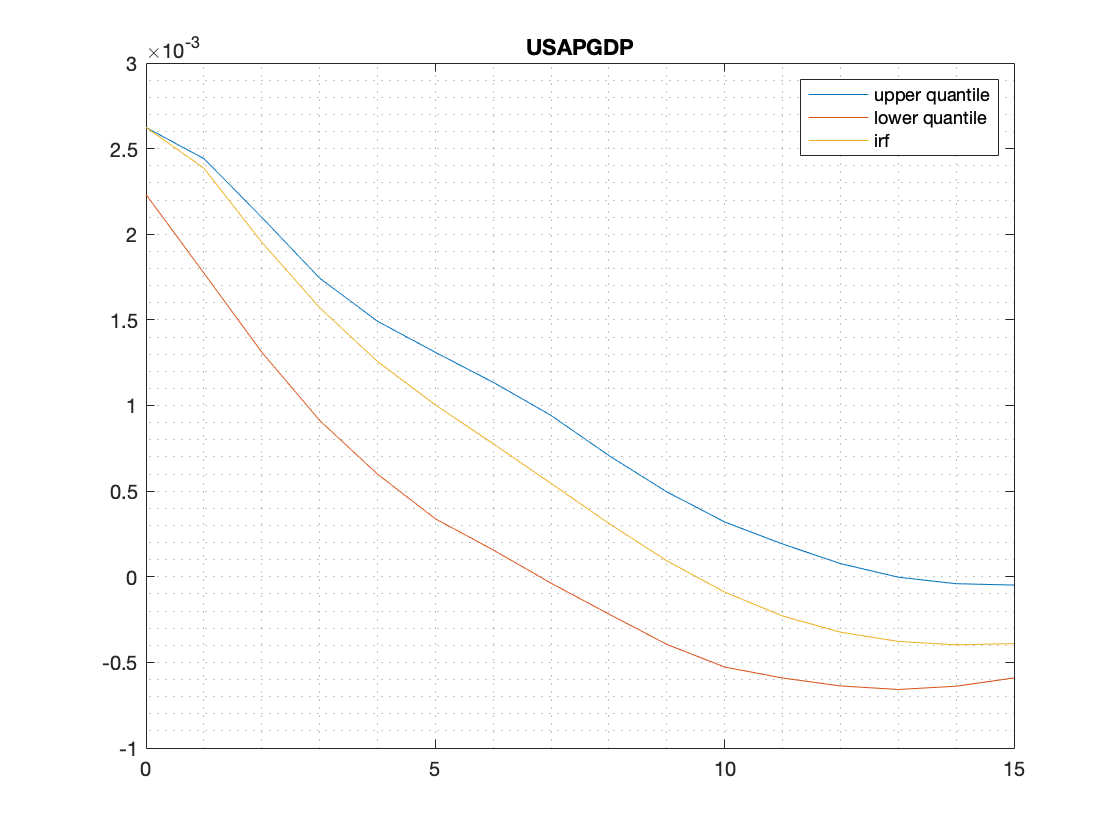
\includegraphics[width=7cm]{ps9fig13_3}
\caption{IRF USAPGDP, Swapped order}
\end{subfigure}
\hfill
\begin{subfigure}[b]{0.45\textwidth}
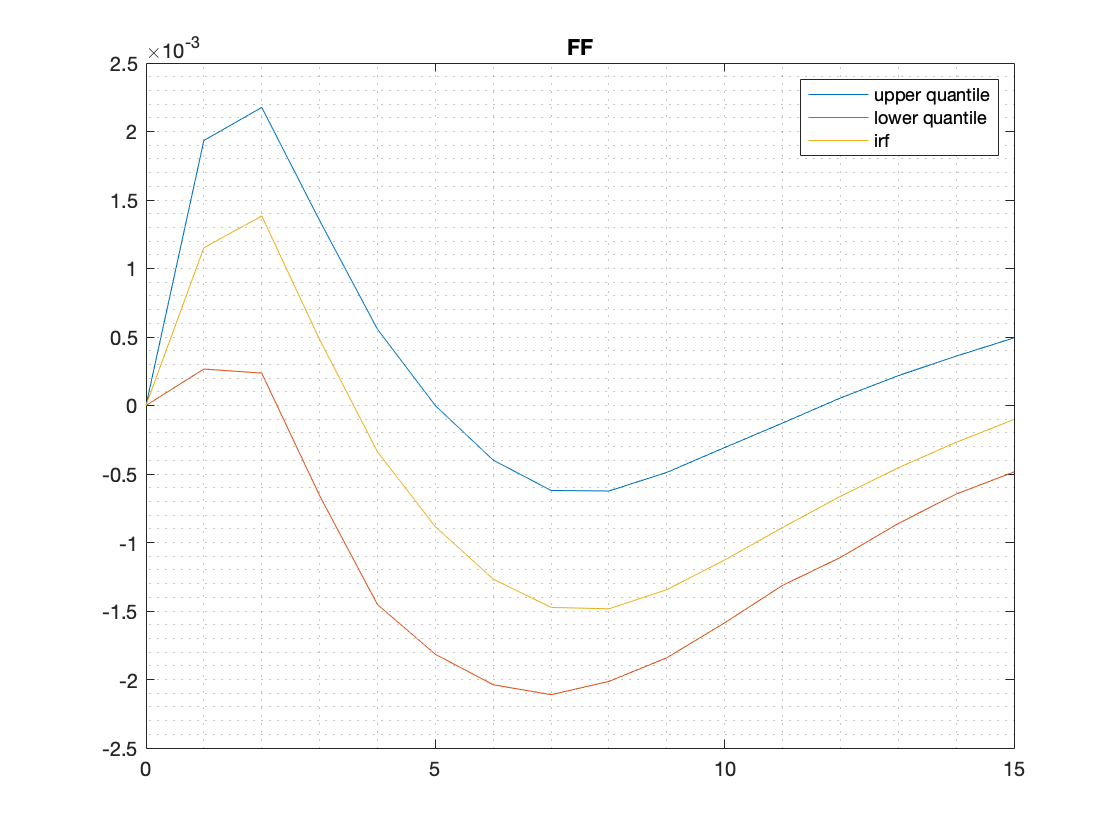
\includegraphics[width=7cm]{ps9fig13_4}
\caption{IRF FF, Swapped order}
\end{subfigure}
\caption{Part 11: Price shock, swapped and normal ordering.}
\end{figure}

\end{document}
	% line of code telling latex that your document is ending. If you leave this out, you'll get an error
